\chapter{Perkembangbiakan Seksual Mamalia}\label{ch:b2:mammal-reproduction}

Sebutir sel telur manusia bergaris tengah sepersepuluh milimeter, sel
terbesar di dalam tubuhnya; sebuah sel sperma adalah sebuah nukleus
dengan baling-baling, satu dari tiga ratus juta yang dilepaskan
sekaligus, dan dari jumlah itu beberapa lusin akan mencapai sel
telurnya dan satu akan memasukinya. Dalam sepekan, sel telur yang telah
dibuahi itu telah menjadi sebuah bola berongga yang membenamkan diri ke
dalam dinding rahim lalu membangun, dari sel luarnya sendiri, sebuah
organ --- \omterm{def:b2:mammal-reproduction:placenta}{plasenta} --- dan lewat organ itu induknya akan
menyuapinya selama sembilan bulan. Lalu ia lahir dan disuapi susu. Tiap
mamalia melakukan hal ini; tidak ada hewan lain yang melakukan
semuanya. Bab ini mengikuti gametnya sampai ke pembuahan, lembaganya
sampai ke \omterm{def:b2:mammal-reproduction:implantation}{implantasi}, dan organismenya melalui kehamilan, kelahiran,
serta laktasi, lalu berakhir dengan bagaimana kedua kelaminnya dibuat.

\section{Gonad dan gamet}

\begin{definition}[Testis dan spermatogenesis]\label{def:b2:mammal-reproduction:testis}
\index{spermatogenesis}\index{tubulus seminiferus}\index{sel Sertoli}\index{sel Leydig}
\emph{Testis} adalah sebuah massa \emph{tubulus seminiferus},
seluruhnya beberapa ratus meter, yang dindingnya membuat sperma; di
antara tubulusnya terletak \emph{sel Leydig}, yang membuat testosteron.
Di dalam dinding tubulusnya, \emph{spermatogonium} pada tepi luarnya
membelah secara mitosis, mempertahankan sebuah populasi punca dan
mengirim sel ke arah dalam; sel itu tumbuh menjadi \emph{spermatosit}
primer, yang menjalani \omterm{def:b2:meiosis-heredity:meiosis}{meiosis} I (menjadi dua spermatosit sekunder) dan
\omterm{def:b2:meiosis-heredity:meiosis}{meiosis} II (menjadi empat \emph{spermatid} \omterm{def:b2:meiosis-heredity:meiosis}{haploid});
spermatidnya melepaskan sebagian besar sitoplasmanya, memadatkan
nukleusnya, menumbuhkan sebuah flagelum, lalu menutupi nukleusnya
dengan \emph{akrosom}, sebuah vesikel enzim, sehingga menjadi
\emph{spermatozoa} yang dilepaskan ke dalam lumennya. \emph{Sel
Sertoli} yang besar merentangi dindingnya, mengasuh sel nutfahnya dan
membentuk, lewat sambungan rapat di antaranya, sebuah
\emph{sawar darah--testis} yang menjauhkan sistem imun dari sel yang
baru muncul pada masa akil balig. Seluruh rangkaiannya memakan
kira-kira \num{64} hari pada seorang pria dan menghasilkan sekitar
$10^{8}$ sperma sehari sejak akil balig sampai usia tua. Sperma
meninggalkan testisnya tanpa gerak lalu matang di dalam
\emph{epididimis} selama dua pekan.
\end{definition}

\begin{omfigure}
\begin{tikzpicture}[every node/.style={font=\scriptsize}]
  % tubule cross-section: concentric layers
  \draw[thick, fill=omExo!15] (0,0) circle (2.5);
  \draw[thick, fill=omExo!8] (0,0) circle (2.2);
  \draw[thick, fill=omDef!10] (0,0) circle (1.6);
  \draw[thick, fill=omProp!12] (0,0) circle (1.0);
  \draw[thick, fill=white] (0,0) circle (0.45);
  % cells
  \foreach \a in {0,30,...,330} \draw[thick, fill=omDef!40] (\a:2.0) circle (0.13);
  \foreach \a in {15,45,...,345} \draw[thick, fill=omDef!70] (\a:1.32) circle (0.16);
  \foreach \a in {0,20,...,340} \draw[thick, fill=omProp!60] (\a:0.75) circle (0.08);
  \foreach \a in {10,40,...,340} \draw[thick, omProp!80!black] (\a:0.45) -- (\a:0.15);
  % Sertoli cell: tall wedge
  \draw[thick, omExo!70!black, fill=omExo!40, opacity=0.6] (100:2.2) .. controls (90:1.6) and (95:0.9) .. (92:0.5) .. controls (80:0.9) and (75:1.6) .. (72:2.2) -- cycle;
  % Leydig cells outside
  \foreach \p in {(2.9,0.8),(3.1,0.3),(2.8,-0.3)} \draw[thick, fill=omThm!40] \p circle (0.14);
  % labels
  \draw (2.0,0) -- (3.6,-0.5) node[right, align=left] {spermatogonium ($2n$)\\pada tepi luarnya};
  \draw (1.32,-0.7) -- (3.6,-1.5) node[right, align=left] {spermatosit primer\\(meiosis I)};
  \draw (0.75,-0.4) -- (3.6,-2.4) node[right, align=left] {spermatid ($n$)};
  \draw (0.3,-0.2) -- (3.6,-3.1) node[right, align=left] {spermatozoa di dalam lumennya};
  \draw (2.95,0.55) -- (3.6,0.6) node[right, align=left] {sel Leydig:\\testosteron};
  \draw (88:1.4) -- (3.6,1.8) node[right, align=left] {sel Sertoli yang merentangi dindingnya};
  \node[anchor=east, align=right] at (-2.7,0) {sebelah luar\\(lamina basal)};
\end{tikzpicture}

{\small Sebuah \omterm{def:b2:mammal-reproduction:testis}{tubulus seminiferus} dalam potongan melintang. Sel
nutfahnya matang dari dinding luarnya (spermatogonium) ke arah dalam
(spermatosit, spermatid, spermatozoa di dalam lumennya), disokong \omterm{def:b2:mammal-reproduction:testis}{sel
Sertoli}; \omterm{def:b2:mammal-reproduction:testis}{sel Leydig} di antara tubulusnya membuat testosteron.}
\end{omfigure}

\begin{omfigure}
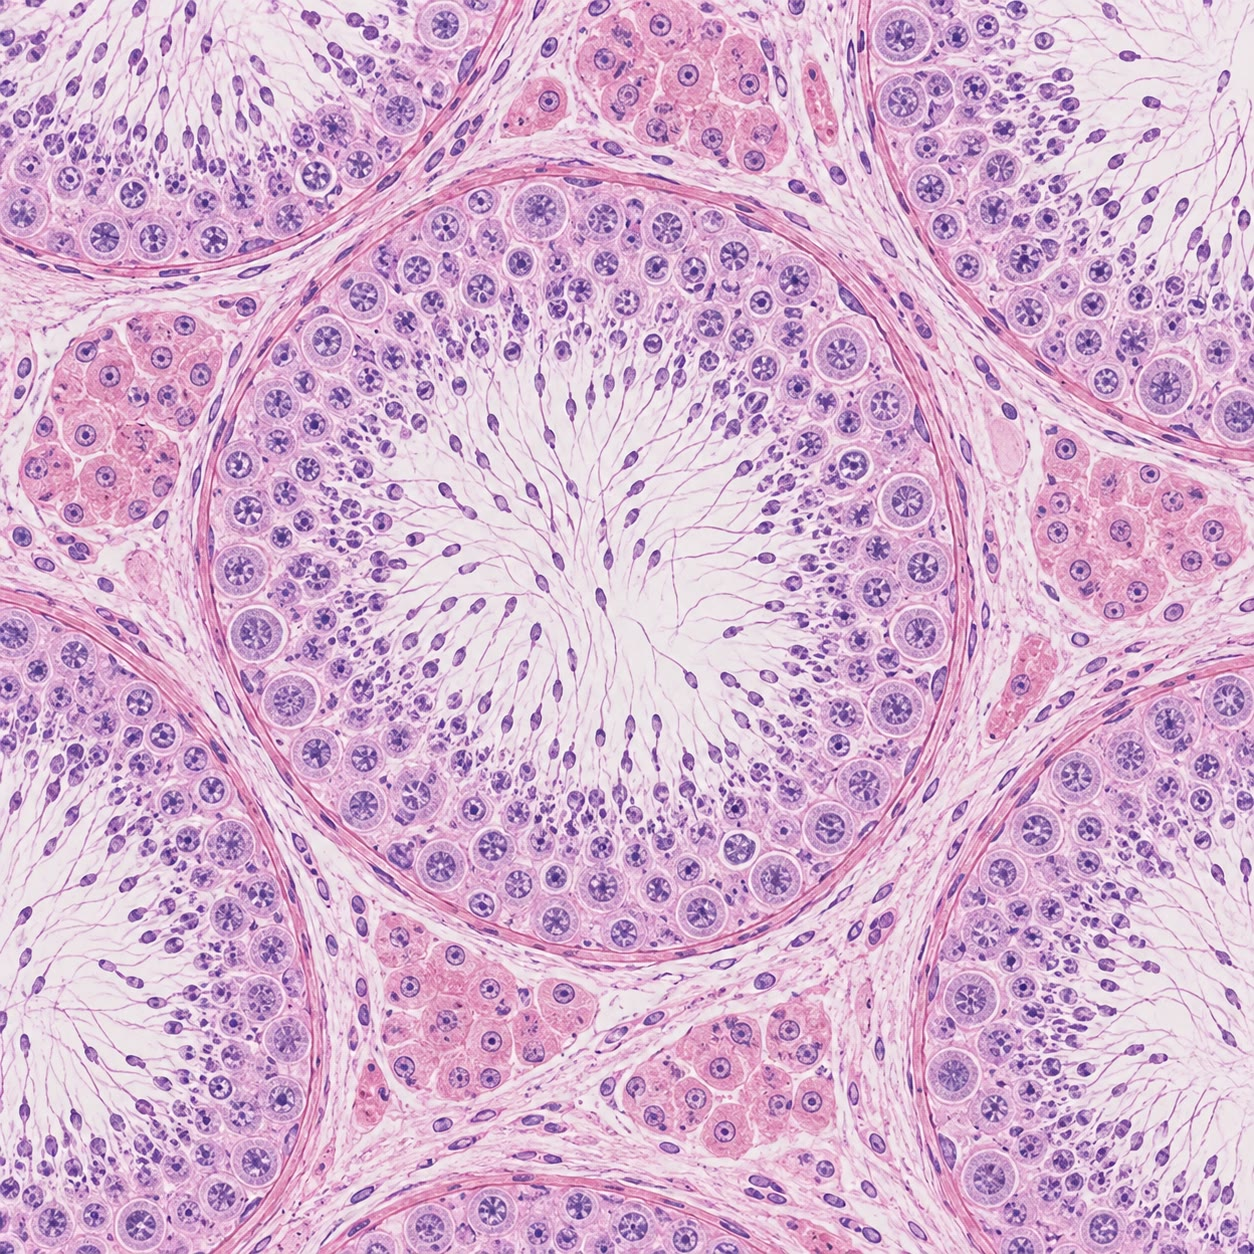
\includegraphics[width=0.42\linewidth]{images/book4/ai/b4-08-testis-histology.jpg}\hspace{0.04\linewidth}
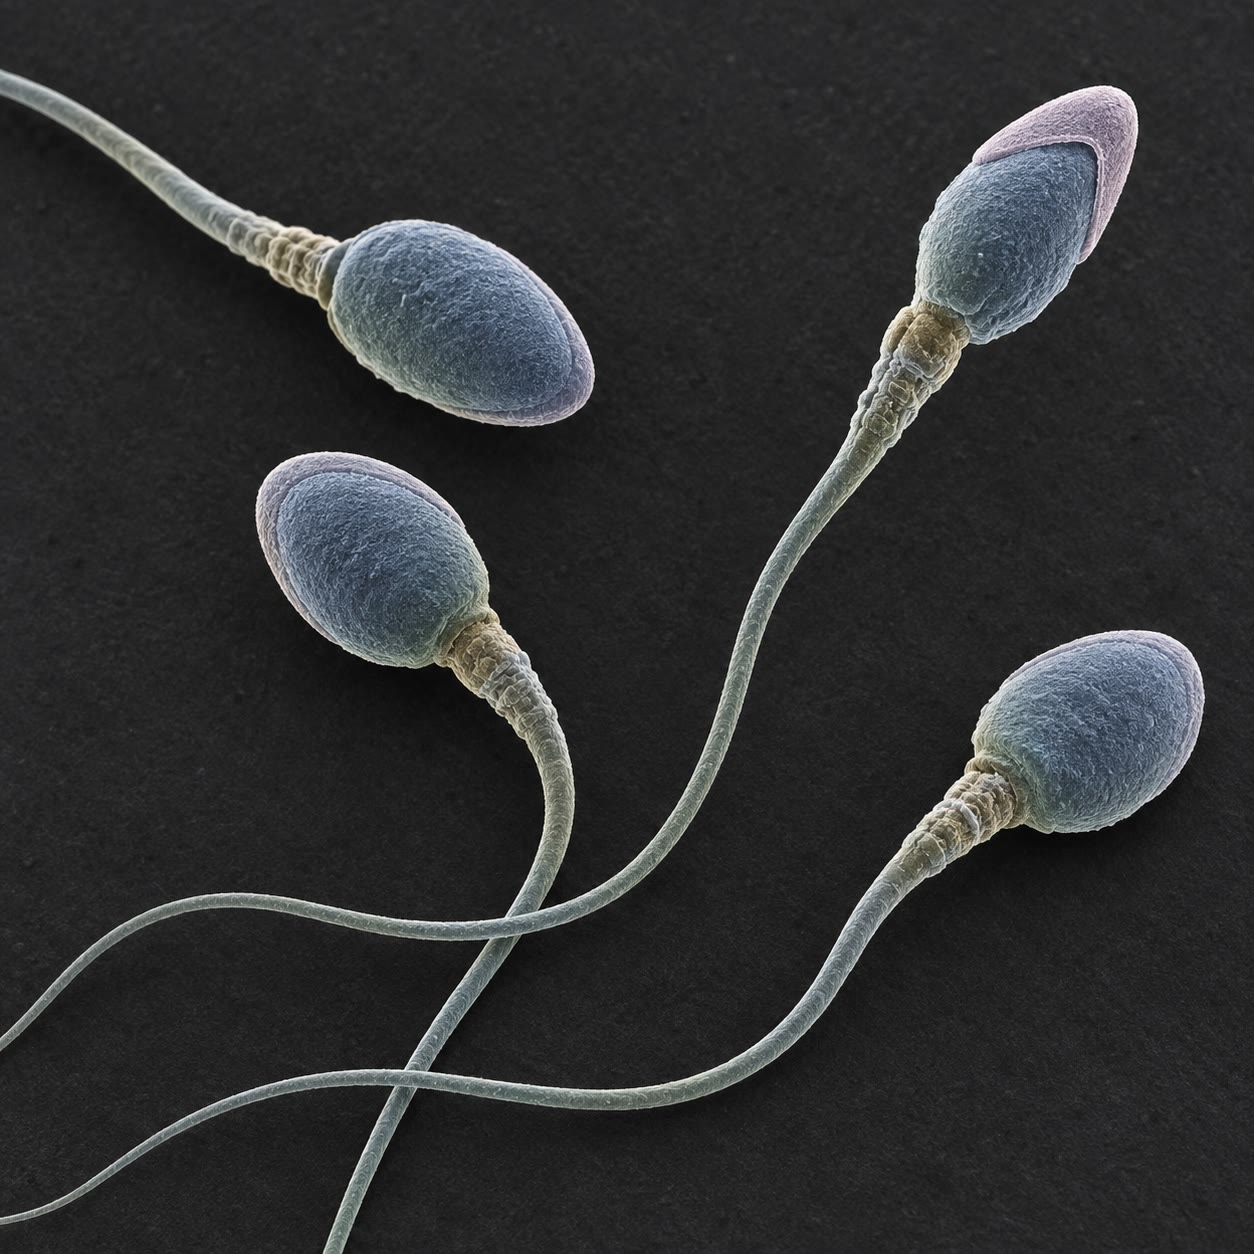
\includegraphics[width=0.42\linewidth]{images/book4/ai/b4-08-sperm-sem.jpg}

{\small Kiri: \omterm{def:b2:mammal-reproduction:testis}{tubulus seminiferus} dalam potongan, sel nutfahnya
berlapis dari dindingnya ke lumennya. Kanan: spermatozoa di bawah
mikroskop elektron payaran, tudung akrosomnya terlihat pada kepalanya.}
\end{omfigure}

\begin{definition}[Ovarium dan oogenesis]\label{def:b2:mammal-reproduction:ovary}
\index{oogenesis}\index{folikel}\index{ovulasi}\index{korpus luteum}
Oogenesis adalah cerminan \omterm{def:b2:mammal-reproduction:testis}{spermatogenesis} dalam hampir tiap seginya.
\emph{Oogonium} berlipat ganda hanya pada janinnya: saat lahir, seorang
anak perempuan mengusung persediaan sekitar sejuta \emph{oosit} primer,
masing-masing terhenti pada \omterm{prop:b2:meiosis-heredity:stages}{profase I} \omterm{def:b2:meiosis-heredity:meiosis}{meiosisnya} dan terbungkus satu
lapis sel --- sebuah \emph{folikel primordial} --- dan tidak pernah ada
yang baru dibuat. Sejak akil balig, tiap bulan sekelompok folikelnya
tumbuh: oositnya membesar, sel \emph{granulosa} di sekelilingnya
berlipat ganda menjadi beberapa lapis, sebuah \emph{teka} luar
terbentuk, sebuah rongga berisi cairan terbuka (\emph{folikel Graaf},
bergaris tengah dua sentimeter), dan biasanya satu folikel saja yang
mencapai \emph{ovulasi}: oositnya, yang baru sekarang menyelesaikan
\omterm{def:b2:meiosis-heredity:meiosis}{meiosis} I lalu terhenti lagi pada metafase II, dikeluarkan bersama
lingkaran sel granulosanya ke dalam saluran telurnya. Folikel yang
telah kosong menjadi \emph{korpus luteum}, sebuah kelenjar progesteron
sementara. \omterm{def:b2:meiosis-heredity:meiosis}{Meiosis} menghasilkan satu sel telur dan tiga badan kutub
yang sangat kecil --- seluruh sitoplasmanya jatuh ke satu sel --- dan
\omterm{def:b2:meiosis-heredity:meiosis}{meiosis} II baru diselesaikan kalau sebuah sperma masuk. Dari sejuta
oositnya, sekitar \num{400} diovulasikan seumur hidup; sisanya merosot
(\emph{atresia}), dan ketika persediaannya habis, sekitar umur lima
puluh, daurnya berhenti: itulah menopause.
\end{definition}

\begin{omfigure}
\begin{tikzpicture}[every node/.style={font=\scriptsize}, >=stealth]
  % timeline of oogenesis vs spermatogenesis
  \draw[thick, ->] (0,3.0) -- (12.6,3.0); \node[anchor=west] at (12.6,3.0) {umur};
  \foreach \x/\l in {0/{janin}, 2.2/{lahir}, 4.6/{akil balig}, 10.2/{$\sim$50 tahun}}
    \draw (\x,3.1) -- (\x,2.9) node[above=0.15cm] {\l};
  % oogenesis line
  \node[anchor=east, omThm] at (-0.2,1.5) {oogenesis};
  \draw[very thick, omThm] (0,1.5) -- (1.6,1.5); \node[above, omThm, align=center] at (0.8,1.55) {oogonium\\berlipat ganda};
  \draw[very thick, omThm, dashed] (1.6,1.5) -- (4.6,1.5); \node[below, omThm] at (3.1,1.45) {terhenti pada profase I};
  \draw[very thick, omThm] (4.6,1.5) -- (10.2,1.5); \node[above, omThm, align=center] at (7.4,1.55) {satu ovulasi tiap bulan;\\meiosis I selesai saat ovulasi, II saat pembuahan};
  \fill[omThm] (10.2,1.5) circle (0.07); \node[below, omThm] at (10.2,1.45) {persediaannya habis};
  % spermatogenesis line
  \node[anchor=east, omDef] at (-0.2,0.3) {spermatogenesis};
  \draw[very thick, omDef, dashed] (0,0.3) -- (4.6,0.3); \node[above, omDef] at (2.3,0.35) {spermatogonium diam};
  \draw[very thick, omDef, ->] (4.6,0.3) -- (12.6,0.3); \node[above, omDef] at (8.6,0.35) {sinambung: $10^{8}$ sperma sehari, 64 hari masing-masing, dari sel punca};
\end{tikzpicture}

{\small Kedua gametogenesisnya dalam waktu. Oosit seluruhnya dibuat
sebelum lahir lalu dilepaskan satu demi satu dari persediaan yang
berhingga; sperma dibuat sinambung dari sel punca sepanjang hidup
dewasanya.}
\end{omfigure}

\begin{omfigure}
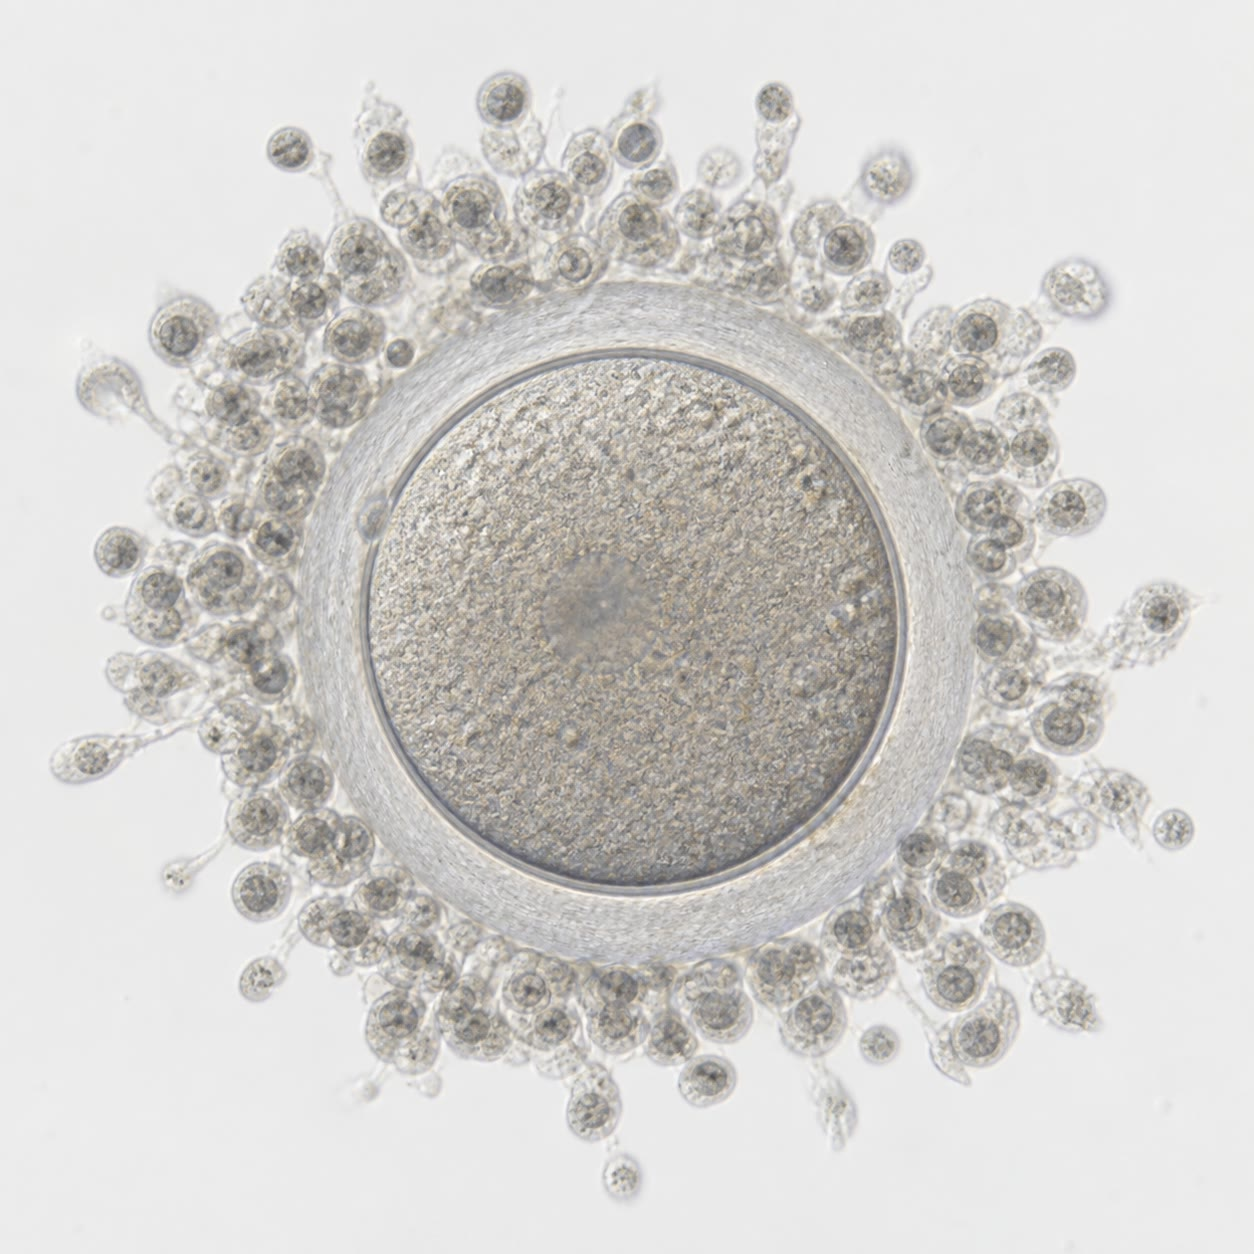
\includegraphics[width=0.46\linewidth]{images/book4/ai/b4-08-oocyte.jpg}

{\small Sebutir oosit yang telah diovulasikan: selnya, mantel
beningnya (\omterm{prop:b2:mammal-reproduction:fertilisation}{zona pelusida}), dan awan sel granulosa yang
meninggalkan \omterm{def:b2:mammal-reproduction:ovary}{folikelnya} bersamanya.}
\end{omfigure}

\section{Pembuahan}

\begin{proposition}[Langkah-langkah pembuahan]\label{prop:b2:mammal-reproduction:fertilisation}
\index{pembuahan!mamalia}\index{reaksi akrosom}%
\index{zona pelusida}\index{reaksi korteks}
Sperma yang disimpankan di dalam vagina --- sekitar $3\times 10^{8}$
--- melintasi lendir serviksnya, disapu naik menyusuri rahim oleh
kerutan rahimnya, dan beberapa ratus mencapai ampula saluran telurnya
dalam waktu sejam, dan di situ sel telurnya menunggu sehari. Dalam
perjalanannya, spermanya menjalani
\emph{kapasitasi}: sekresi saluran betinanya melucuti protein pelapis
membrannya lalu menjadikannya sangat giat. Pada sel telurnya, sebuah
sperma mendorong lewat sel granulosanya, mengikat sebuah glikoprotein
\emph{\omterm{prop:b2:mammal-reproduction:fertilisation}{zona pelusida}}, lalu menjalani \emph{\omterm{prop:b2:mammal-reproduction:fertilisation}{reaksi akrosom}}, dan
melepaskan enzim yang mencerna sebuah jalan menembus zonanya;
membrannya melebur dengan membran sel telurnya, dan nukleus spermanya
masuk. Sel telurnya menanggapinya dalam hitungan detik: kalsium
menyapu melintasinya, dan butiran korteksnya melepaskan enzim yang
mengeraskan zonanya serta melucuti reseptor spermanya --- itulah
\emph{\omterm{prop:b2:mammal-reproduction:fertilisation}{reaksi korteks}}, yakni penghadang polispermi.
Sel telurnya lalu menyelesaikan \omterm{def:b2:meiosis-heredity:meiosis}{meiosis} II, melepaskan badan kutub
kedua, dan kedua \emph{pronukleus} \omterm{def:b2:meiosis-heredity:meiosis}{haploidnya} mereplikasi DNA-nya, mendekat,
lalu memasuki mitosis pertamanya: zigotnya berumur sehari. Kekhususan
spesiesnya terletak pada protein zonanya, dan itulah sebabnya sperma
mencit tidak memasuki sel telur manusia.
\end{proposition}
\begin{proof}[Bukti eksperimental]
Edwards dan Steptoe (1978) membuahi sebutir oosit manusia, yang
diambil dari ovariumnya sesaat sebelum \omterm{def:b2:mammal-reproduction:ovary}{ovulasi}, dengan sperma
terkapasitasi di dalam cawan, membiakkan lembaganya sampai delapan sel,
lalu mengembalikannya ke dalam rahim, dan di situ ia berimplantasi
lalu lahir: itulah pembuahan di luar tubuh. Tiap langkah rangkaian di atas
pertama-tama dipecahkan pada bulu babi laut dan mencit, tempat
peleburannya, gelombang kalsiumnya, dan pelepasan butiran korteksnya
dapat disaksikan; pada mencit, membuang satu glikoprotein zonanya (ZP2
atau ZP3) lewat \omterm{def:b2:genome-diversification:mutation}{mutasi} meninggalkan sel telur yang tidak dapat
diikat sperma.
\end{proof}

\begin{theorem}[Mengapa satu sel telur membutuhkan berjuta sperma]\label{thm:b2:mammal-reproduction:poisson}
\index{polispermi}
Kalau, dari $N$ sperma yang disimpankan, masing-masing mencapai
permukaan sel telurnya secara bebas dengan peluang kecil $\pi$, cacah
yang tiba berdistribusi Poisson dengan purata $m = N\pi$ dan peluang
bahwa sedikitnya satu tiba adalah
\[
P = 1 - e^{-m}.
\]
Dengan $N = 3\times 10^{8}$ dan $\pi \approx 10^{-8}$, $m \approx 3$
dan $P \approx 0.95$; dengan $N = 2\times 10^{7}$ (ambang klinis
cacah sperma yang rendah), $m = 0.2$ dan $P = 0.18$. Aritmetika yang
sama menunjukkan mengapa penghadang polispermi tak tergantikan: ketika
$P$ tinggi, beberapa sperma tiba dalam selang beberapa detik satu sama
lain, dan sel telur yang dimasuki dua sperma akan triploid lalu mati.
\end{theorem}
\begin{proof}
Tiap spermanya adalah percobaan bebas dengan peluang berhasil $\pi$;
cacah keberhasilannya binomial, yang bagi $N$ besar dan $\pi$ kecil
berdistribusi Poisson dengan purata $N\pi$. Peluang nol
keberhasilan adalah $e^{-m}$, sehingga peluang sedikitnya satu adalah
$1 - e^{-m}$; peluang dua atau lebih adalah $1 - e^{-m}(1 + m)$,
kira-kira $0.8$ bagi $m = 3$.
\end{proof}

\begin{omfigure}
\begin{tikzpicture}[every node/.style={font=\scriptsize}, >=stealth]
  \foreach \x/\lab in {0/{1. sperma mengikat\\zonanya}, 3.3/{2. reaksi akrosom:\\enzim memotong sebuah jalan}, 6.6/{3. membrannya melebur;\\gelombang kalsium}, 9.9/{4. reaksi korteks:\\zonanya mengeras,\\meiosis II selesai}} {
    \begin{scope}[xshift=\x cm]
      \draw[thick, fill=omThm!8] (0,0) circle (0.9);
      \draw[thick, omExo!70!black] (0,0) circle (1.15);
      \node[below, align=center] at (0,-1.3) {\lab};
    \end{scope}
  }
  % stage 1: sperm at zona
  \draw[thick, fill=omDef!50] (-1.45,0.1) ellipse (0.18 and 0.11); \draw[thick, omDef] (-1.63,0.1) .. controls (-2.0,0.4) and (-2.2,-0.2) .. (-2.5,0.1);
  % stage 2: sperm digging through zona
  \begin{scope}[xshift=3.3cm]
    \fill[white] (-1.2,0.0) circle (0.12);
    \draw[thick, fill=omDef!50] (-1.05,0.05) ellipse (0.18 and 0.11); \draw[thick, omDef] (-1.23,0.05) .. controls (-1.6,0.35) and (-1.8,-0.25) .. (-2.1,0.05);
    \foreach \a in {150,170,190,210} \draw[omProp, thick] (-1.2,0.0) -- ++(\a:0.25);
  \end{scope}
  % stage 3: fused, calcium wave
  \begin{scope}[xshift=6.6cm]
    \fill[white] (-1.15,0.0) circle (0.12);
    \draw[thick, fill=omDef!50] (-0.75,0.0) ellipse (0.18 and 0.11);
    \draw[thick, omDef] (-0.93,0.0) .. controls (-1.3,0.3) and (-1.5,-0.3) .. (-1.8,0.0);
    \foreach \r in {0.35,0.55,0.75} \draw[omProp, thick] (-0.75,0) ++(-60:\r) arc (-60:60:\r);
  \end{scope}
  % stage 4: hardened zona, polar body, pronuclei
  \begin{scope}[xshift=9.9cm]
    \draw[very thick, omExo!70!black] (0,0) circle (1.15);
    \draw[thick, fill=omDef!30] (-0.25,0.05) circle (0.2); \draw[thick, fill=omThm!30] (0.25,0.05) circle (0.2);
    \draw[thick, fill=omThm!20] (0.55,0.95) circle (0.12);
    \node[anchor=west] at (1.2,0.9) {badan kutub};
    \draw (0.45,0.05) -- (1.2,-0.35); \node[anchor=west] at (1.2,-0.35) {dua pronukleus};
  \end{scope}
\end{tikzpicture}

{\small Pembuahan dalam empat langkah: pengikatan pada zonanya,
\omterm{prop:b2:mammal-reproduction:fertilisation}{reaksi akrosom}, peleburan dan gelombang kalsiumnya, serta \omterm{prop:b2:mammal-reproduction:fertilisation}{reaksi
korteks} yang menutup sel telurnya bagi sperma lain sembari ia
menyelesaikan \omterm{def:b2:meiosis-heredity:meiosis}{meiosis}.}
\end{omfigure}

\section{Implantasi dan plasenta}

\begin{definition}[Pembelahan, blastosista, implantasi]\label{def:b2:mammal-reproduction:implantation}
\index{blastosista}\index{trofoblas}\index{massa sel dalam}\index{implantasi}
Zigotnya membelah tiap dua belas sampai dua puluh jam tanpa tumbuh
(\emph{pembelahan}) sembari dipindahkan menyusuri saluran telurnya: dua
sel, empat, delapan, sebuah bola padat berisi enam belas
(\emph{morula}), dan pada hari kelima sebuah \emph{blastosista}
berisi kira-kira seratus sel: sebuah lapisan luar, yaitu
\emph{trofoblas}, mengelilingi sebuah rongga, dengan segumpal sel di
satu sisinya, yaitu \emph{massa sel dalam}. Trofoblasnya akan
membangun \omterm{def:b2:mammal-reproduction:placenta}{plasenta} dan selaputnya; massa sel dalamnya akan menjadi
lembaganya --- dan, kalau diambil pada tahap ini, memberi sel punca
lembaga. Pada hari keenam, blastosistanya menetas dari zonanya,
melekat pada pelapis rahimnya, dan trofoblasnya menyerbunya: selnya
melebur menjadi sebuah muka berinti banyak yang mencerna jaringan
induknya lalu membuka kapiler induknya, sehingga pada hari kedua belas
lembaganya terbenam di dalam dindingnya dan bermandi darah induknya.
Inilah \emph{implantasi}. Ia hanya berhasil di dalam rahim yang telah
disiapkan progesteron, dalam sebuah jendela beberapa hari; kira-kira
separuh dari semua pembuahan manusia gagal sebelum atau pada langkah
ini, biasanya karena kekeliruan kromosom sel telurnya.
\end{definition}

\begin{omfigure}
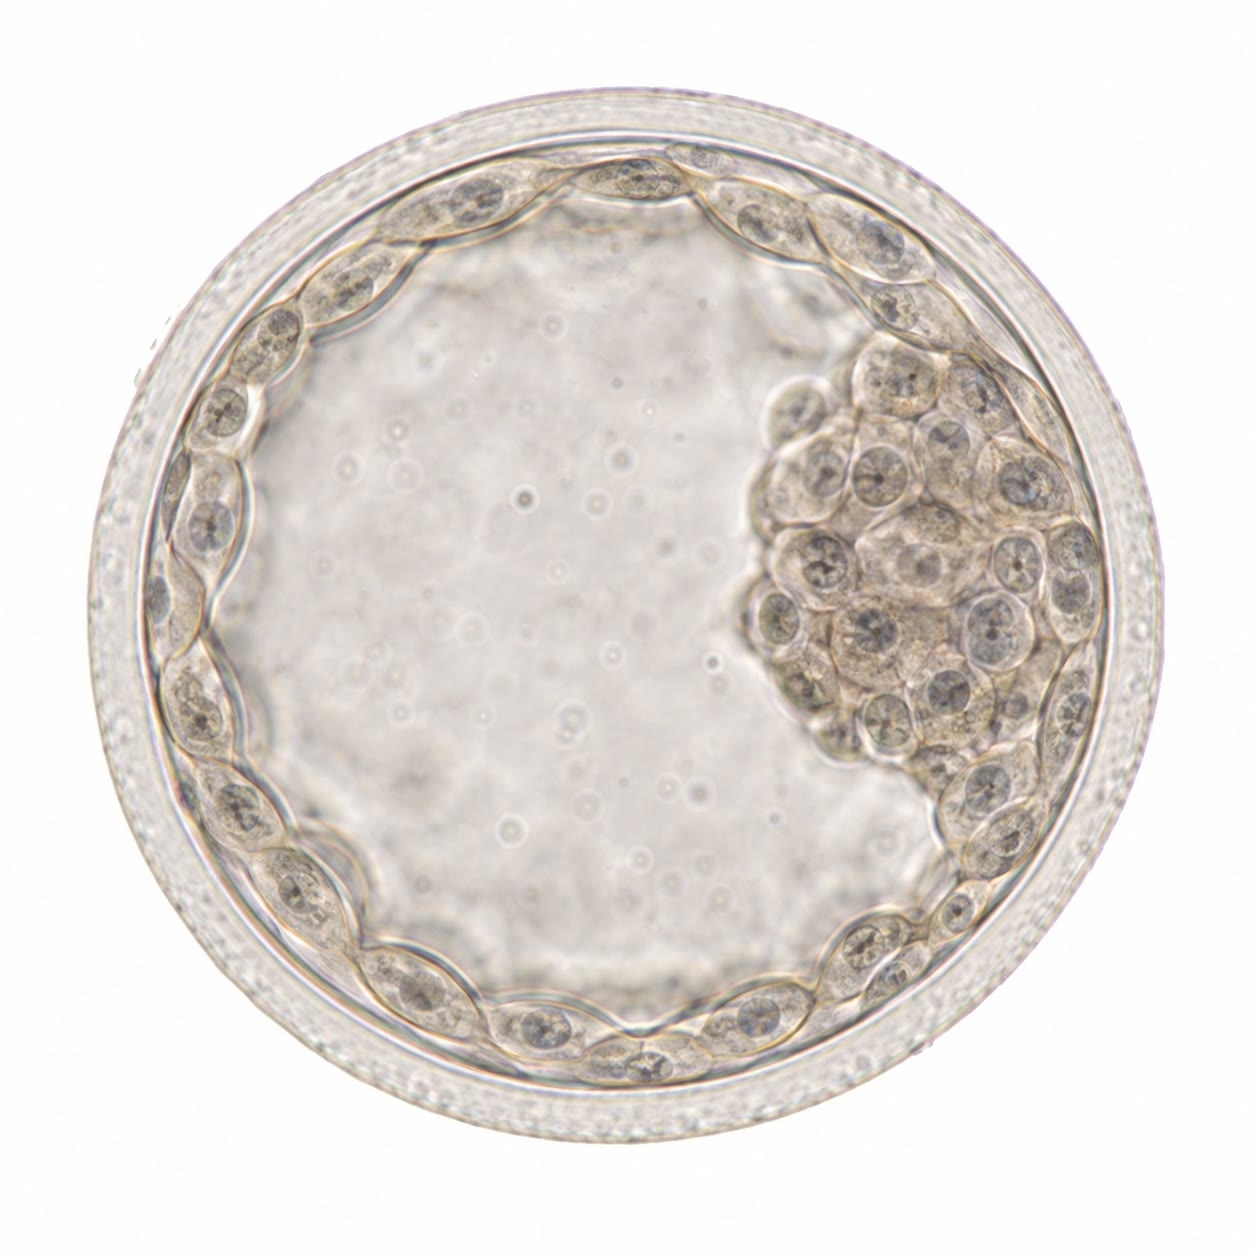
\includegraphics[width=0.42\linewidth]{images/book4/ai/b4-08-blastocyst.jpg}

{\small Sebuah \omterm{def:b2:mammal-reproduction:implantation}{blastosista} pada hari kelima: \omterm{def:b2:mammal-reproduction:implantation}{trofoblas} luarnya
mengelilingi rongganya, dan \omterm{def:b2:mammal-reproduction:implantation}{massa sel dalamnya} --- lembaga masa depan
--- berada di satu sisinya.}
\end{omfigure}

\begin{definition}[Plasenta]\label{def:b2:mammal-reproduction:placenta}
\index{plasenta}\index{vilus korion}\index{tali pusat}
\emph{Plasenta} adalah sebuah organ yang dibuat bersama-sama oleh
lembaganya (korion, dari \omterm{def:b2:mammal-reproduction:implantation}{trofoblasnya}) dan induknya (pelapis
rahimnya). \emph{Vilus korion} yang menyerupai jari, bercabang menjadi
sebuah permukaan seluas sekitar \qty{12}{m^2} pada akhir kehamilan,
bergantung di dalam danau darah induknya yang diantarkan arteri
rahimnya setengah liter tiap menit; di dalam tiap vilusnya mengalir
kapiler janinnya, yang tersambung kepada janinnya lewat kedua arteri
dan satu vena \emph{tali pusat}. Kedua darahnya tidak pernah bercampur:
keduanya dipisahkan dinding vilusnya, yaitu beberapa mikrometer
\omterm{def:b2:mammal-reproduction:implantation}{trofoblas} dan endotelium kapiler, dan menyeberanginya oksigen,
$\mathrm{CO_2}$, air, urea, serta molekul yang larut lemak berdifusi,
glukosa dan asam amino diangkut pengangkut, dan antibodi induknya
(IgG) diseberangkan reseptor, sehingga memberi bayinya kekebalan
bulan-bulan pertamanya. Plasentanya juga sebuah kelenjar: sejak
hari-hari pertama, \omterm{def:b2:mammal-reproduction:implantation}{trofoblasnya} menyekresikan \emph{gonadotropin
korion manusia} (hCG), yang menjaga \omterm{def:b2:mammal-reproduction:ovary}{korpus luteumnya} tetap
membuat progesteron, dan sejak bulan ketiga plasentanya sendiri membuat
progesteron dan estrogen yang mempertahankan kehamilannya
(\cref{ch:b2:reproductive-hormones}). Ia, pada dasarnya, adalah sebuah
paru-paru, sebuah usus, sebuah ginjal, dan sebuah kelenjar endokrin
yang ditumbuhkan selama sembilan bulan lalu dibuang saat lahir.
\end{definition}

\begin{omfigure}
\begin{tikzpicture}[every node/.style={font=\scriptsize}, >=stealth]
  % maternal blood space
  \fill[omThm!12] (0,0) rectangle (8,3.6);
  \node[omThm!80!black, align=center] at (1.1,2.6) {darah induknya\\(ruang\\antarvilus)};
  % uterine wall at bottom
  \fill[omExo!30] (0,-0.6) rectangle (8,0); \node at (4,-0.3) {dinding rahim (induknya)};
  \draw[->, thick, omThm] (1.0,-0.6) -- (1.0,0.6); \node[omThm, anchor=west] at (1.05,0.3) {arteri spiral};
  \draw[->, thick, omDef!60!black] (7.0,0.6) -- (7.0,-0.6); \node[omDef!60!black, anchor=east] at (6.95,0.3) {vena rahim};
  % chorionic plate at top
  \fill[omDef!20] (0,3.6) rectangle (8,4.4); \node at (4,4.0) {lempeng korion (janinnya)};
  % villi hanging down
  \foreach \x in {2.6,4.2,5.8} {
    \draw[thick, fill=omDef!8] (\x-0.35,3.6) -- (\x-0.4,1.4) .. controls (\x-0.4,0.9) and (\x+0.4,0.9) .. (\x+0.4,1.4) -- (\x+0.35,3.6);
    \draw[thick, omThm!70!black] (\x-0.15,3.6) -- (\x-0.15,1.5) .. controls (\x-0.15,1.25) and (\x+0.15,1.25) .. (\x+0.15,1.5) -- (\x+0.15,3.6);
    \foreach \y in {2.0,2.7} { \draw[thick, fill=omDef!8] (\x-0.4,\y) .. controls (\x-0.9,\y+0.1) and (\x-0.9,\y-0.4) .. (\x-0.4,\y-0.3); }
  }
  % umbilical vessels
  \draw[very thick, omThm!70!black] (4.2,4.4) -- (4.2,5.0) node[above, align=center] {vena pusat (ke janinnya)\\dan arterinya};
  \draw[very thick, omDef!60!black] (3.9,4.4) -- (3.9,5.0); \draw[very thick, omDef!60!black] (4.5,4.4) -- (4.5,5.0);
  % exchange arrows
  \draw[<->, thick] (3.0,2.2) -- (3.75,2.2); \node[anchor=west, align=left] at (8.3,1.5) {menyeberangi dindingnya: \textcolor{omThm}{O$_2$, glukosa,}\\\textcolor{omThm}{asam amino, IgG} menuju janinnya;\\\textcolor{omDef!60!black}{CO$_2$, urea} menuju induknya};
  \node[anchor=west, align=left] at (8.3,3.0) {dinding vilusnya: trofoblas\\+ endotelium kapiler janinnya,\\beberapa mikrometer};
  \draw (6.2,2.5) -- (8.3,3.0);
\end{tikzpicture}

{\small \omterm{def:b2:mammal-reproduction:placenta}{Plasenta}: vilus janinnya, yang mengusung kapiler janinnya,
bergantung di dalam sebuah ruang yang terisi darah induknya dari arteri
spiralnya. Kedua darahnya bertukar menyeberangi dinding vilusnya dan
tidak pernah bercampur.}
\end{omfigure}

\begin{theorem}[Pertukaran menyeberangi plasenta]\label{thm:b2:mammal-reproduction:fick}
\index{hukum Fick!plasenta}
Sebuah gas yang menyeberangi membran berluas $A$ dan bertebal $d$
bergerak pada laju $J = K\,A\,\Delta P/d$, dengan $\Delta P$ sebagai
selisih tekanan parsialnya dan $K$ sebagai keterlewatan jaringannya.
Bagi oksigen di dalam jaringan $K \approx \qty{3e-8}{mL/(cm.min.mmHg)}$; dengan $A =
\qty{12}{m^2}$, $d = \qty{3.5}{\micro m}$ dan $\Delta P =
\qty{20}{mmHg}$ (induknya \qty{40}{mmHg} di dalam ruang antarvilusnya
terhadap \qty{20}{mmHg} di dalam arteri pusatnya), \omterm{def:b2:mammal-reproduction:placenta}{plasentanya} dapat
melewatkan kira-kira \qty{200}{mL} oksigen tiap menit, yaitu sekitar
delapan kali \qty{25}{mL/min} yang dipakai janin cukup bulan. Maka
pemindahan oksigennya dibatasi bukan oleh difusinya melainkan oleh
aliran darahnya; janinnya bekerja pada tekanan oksigen yang rendah lalu
mengimbanginya dengan hemoglobin berdaya ikat lebih tinggi dan cacah
sel darah merah yang lebih besar.
\end{theorem}
\begin{proof}
Hukum Fick menyatakan bahwa fluksnya sebanding dengan landaiannya
$\Delta P/d$ dan dengan luasnya; tetapan $K$ menyerap kelarutan dan
koefisien difusi gasnya di dalam jaringan. Secara angka:
$3\times 10^{-8}\times 1.2\times 10^{5}\times 20/(3.5\times 10^{-4})
= \qty{206}{mL/min}$ dengan $A$ dalam \unit{cm^2} dan $d$ dalam \unit{cm}.
Permintaan janinnya kira-kira \qty{7}{mL} tiap kilogram tiap menit bagi
\qty{3.5}{kg}.
\end{proof}

\section{Kehamilan, kelahiran, dan laktasi}

\begin{proposition}[Kehamilan dan kelahiran]\label{prop:b2:mammal-reproduction:birth}
\index{kehamilan}\index{kelahiran}\index{oksitosin}
Kehamilan berlangsung \num{20} hari pada mencit, \num{280} hari pada
manusia, \num{660} hari pada gajah --- kira-kira sebagai pangkat
seperempat massa tubuhnya, dengan primata yang lambat bagi ukurannya.
Ia dipertahankan progesteron, yang menjaga otot rahimnya tetap tenang
dan serviksnya tertutup. Kelahiran (\emph{partus}) dipicu janinnya
sendiri: kortisol
adrenalnya, yang naik menjelang cukup bulan, mengalihkan \omterm{def:b2:mammal-reproduction:placenta}{plasentanya}
dari progesteron ke estrogen, yang memasangi rahimnya dengan reseptor
oksitosin serta sambungan renggang lalu memulai pelepasan
prostaglandin. Kemudian sebuah \emph{umpan balik positif} mengambil
alih: kepalanya menekan serviksnya, saraf inderanya mengisyaratkannya
kepada hipotalamusnya, \emph{oksitosin} dilepaskan dari hipofisis
posteriornya, rahimnya berkerut, kepalanya menekan lebih keras; gelungnya
meningkat sampai kelahirannya, dan sesudah itu rangsangannya berakhir
lalu gelungnya berhenti --- salah satu dari sedikit umpan balik positif
dalam fisiologi, dan salah satu yang harus berakhir pada sebuah
peristiwa. \omterm{def:b2:mammal-reproduction:placenta}{Plasentanya} dilahirkan beberapa menit kemudian.
\end{proposition}
\begin{proof}[Bukti eksperimental]
Ferguson (1941) menunjukkan pada kelinci bahwa merenggangkan serviksnya
membangkitkan kerutan rahim dan bahwa memotong sumsum tulang
belakangnya atau membuang hipofisis posteriornya meniadakan
tanggapannya: sebuah refleks neuroendokrin dari serviks ke hipofisis ke
rahim. Oksitosin, yang diisolasi dan disintesis du Vigneaud pada 1953,
kini menjadi obat baku untuk mengimbas persalinan.
\end{proof}

\begin{proposition}[Laktasi]\label{prop:b2:mammal-reproduction:lactation}
\index{laktasi}\index{prolaktin}\index{susu}
Kelenjar susu, yaitu kelenjar keringat yang berubah bentuk, dibangun
selama kehamilan oleh estrogen, progesteron, dan prolaktin tetapi
ditahan dari menyekresi oleh progesteron; ketika \omterm{def:b2:mammal-reproduction:placenta}{plasentanya} pergi,
progesteronnya turun dan, di bawah \emph{prolaktin} dari hipofisis
anteriornya, alveolusnya mulai membuat susu. Dua refleks menjalankan
prosesnya: mengisap merangsang pelepasan prolaktin (yang
mempertahankan sintesisnya dan menekan \omterm{def:b2:mammal-reproduction:ovary}{ovulasinya}) dan pelepasan
oksitosin (yang mengerutkan sel di sekeliling alveolusnya lalu
memancarkan susunya). Susu manusia mengusung kira-kira \qty{7}{\%}
laktosa, \qty{4}{\%} lemak, \qty{1}{\%} protein, dan
\qty{2.9}{kJ/mL}; \emph{kolostrum} hari-hari pertamanya kaya antibodi
(IgA) yang melapisi usus bayinya. Seorang ibu membuat kira-kira
\qty{750}{mL} sehari, dengan ongkos sekitar \qty{2.5}{MJ} --- seperempat
makanannya --- selama berbulan-bulan; laktasi adalah bagian
perkembangbiakan mamalia yang paling mahal dan bagian yang menamai
kelasnya.
\end{proposition}

\section{Membuat kedua kelaminnya}

\begin{proposition}[Penentuan dan diferensiasi kelamin]\label{prop:b2:mammal-reproduction:sex}
\index{SRY}\index{hormon anti-Müller}\index{diferensiasi kelamin}
Sampai pekan keenam, sebuah lembaga manusia kelamin apa pun memiliki
perlengkapan yang sama: sebuah gonad yang tak tentu, dua pasang saluran
(\emph{Wolff} dan \emph{Müller}), dan alat kelamin luar yang netral.
Gen \emph{SRY} pada kromosom Y menyala di dalam gonadnya lalu
mengubahnya menjadi sebuah testis; tanpanya gonadnya menjadi sebuah
ovarium. \omterm{def:b2:mammal-reproduction:testis}{Testis} janinnya lalu mengerjakan dua hal: \omterm{def:b2:mammal-reproduction:testis}{sel Sertolinya}
menyekresikan \emph{\omterm{prop:b2:mammal-reproduction:sex}{hormon anti-Müller}}, yang membuat saluran Müllernya
menyusut, dan \omterm{def:b2:mammal-reproduction:testis}{sel Leydignya} menyekresikan \emph{testosteron}, yang
mempertahankan saluran Wolffnya (bakal epididimis, vas deferens, dan
vesikula seminalis) dan, sesudah diubah menjadi dihidrotestosteron,
membentuk alat kelamin luarnya menjadi penis dan skrotum. Tanpa kedua
isyarat itu, saluran Wolffnya menyusut, saluran Müllernya menjadi
saluran telur, rahim, dan vagina bagian atasnya, serta alat kelaminnya
berkembang sebagai betina. Jalan betinanya adalah jalan yang ditempuh
ketika tidak ada yang dikatakan: jalan jantannya harus dipaksakan
secara aktif oleh testisnya, dan tiap langkah tempat pemaksaannya gagal
--- SRY yang mutan, sebuah reseptor hormon yang hilang --- memberi
individu XY dengan tubuh betina atau antara.
\end{proposition}
\begin{proof}[Bukti eksperimental]
Jost (1947) membuang gonad janin kelinci di dalam rahimnya sebelum
salurannya berdiferensiasi: janin yang dikebiri, kelamin kromosom apa
pun, mengembangkan rahim, saluran telur, dan alat kelamin betina.
Sebutir hablur testosteron yang ditanam pada janin yang dikebiri
mempertahankan saluran Wolffnya pada sisi itu tetapi tidak membuang
saluran Müllernya; sebuah testis janin yang dicangkokkan mengerjakan
keduanya, pada sisinya sendiri: testisnya pastilah membuat sebuah
faktor kedua, yang saat itu belum dikenal, untuk menekan saluran
betinanya, yang tiga puluh tahun kemudian dikenali sebagai \omterm{prop:b2:mammal-reproduction:sex}{hormon
anti-Müller}. Kemudian pengaruh pembalik kelamin dari sekeping kecil
kromosom Y memakukan sakelarnya pada \emph{SRY} (1990), dan seekor
mencit yang dibuat XX dengan gen \emph{Sry} saja berkembang sebagai
jantan.
\end{proof}

\begin{omfigure}
\begin{tikzpicture}[every node/.style={font=\scriptsize}, >=stealth]
  \node[draw, rounded corners, fill=omExo!25, align=center] (g) at (0,0) {gonad tak tentu\\dua sistem saluran};
  \node[draw, rounded corners, fill=omDef!15, align=center] (t) at (4.2,1.4) {testis\\(\emph{SRY} hadir)};
  \node[draw, rounded corners, fill=omThm!15, align=center] (o) at (4.2,-1.4) {ovarium\\(tanpa \emph{SRY})};
  \node[draw, rounded corners, fill=omDef!15, align=center] (amh) at (8.6,2.3) {AMH: saluran Müller menyusut};
  \node[draw, rounded corners, fill=omDef!15, align=center] (tst) at (8.6,0.6) {testosteron: saluran Wolff dipertahankan;\\DHT: alat kelamin luar jantan};
  \node[draw, rounded corners, fill=omThm!15, align=center] (f) at (8.6,-1.4) {tanpa isyarat: saluran Wolff menyusut,\\saluran Müller $\to$ saluran telur, rahim;\\alat kelamin betina};
  \draw[->, thick] (g) -- (t); \draw[->, thick] (g) -- (o);
  \draw[->, thick] (t) -- (amh); \draw[->, thick] (t) -- (tst); \draw[->, thick] (o) -- (f);
\end{tikzpicture}

{\small \omterm{prop:b2:mammal-reproduction:sex}{Diferensiasi kelamin}: testisnya, yang dibuat \emph{SRY},
memaksakan jalan jantannya dengan dua hormon; tanpa keduanya tubuhnya
berkembang sebagai betina.}
\end{omfigure}

\section{Latihan}

\begin{exercise}[$\star$]\label{exo:b2:mammal-reproduction:1}
Bandingkanlah \omterm{def:b2:mammal-reproduction:testis}{spermatogenesis} dan \omterm{def:b2:mammal-reproduction:ovary}{oogenesis}: kapan sel puncanya
membelah, berapa gamet yang dihasilkan satu \omterm{def:b2:meiosis-heredity:meiosis}{meiosis}, berapa lama sebuah
gamet dibuat, di mana penghentiannya, dan berapa gamet yang dihasilkan
seumur hidup.
\end{exercise}

\begin{exercise}[$\star$]\label{exo:b2:mammal-reproduction:2}
Daftarkan langkah pembuahan dari tibanya sebuah sperma pada zonanya
sampai mitosis pertamanya, lalu katakan langkah mana yang menghadang
polispermi.
\end{exercise}

\begin{exercise}[$\star$]\label{exo:b2:mammal-reproduction:3}
Sebutkan kedua populasi sel \omterm{def:b2:mammal-reproduction:implantation}{blastosistanya} dan nasib
masing-masingnya. Pada hari keberapa \omterm{def:b2:mammal-reproduction:implantation}{implantasinya} mulai, dan hormon
apa yang pastilah telah menyiapkan rahimnya?
\end{exercise}

\begin{exercise}[$\star$]\label{exo:b2:mammal-reproduction:4}
Bagi tiap hal berikut, katakan apakah ia menyeberangi \omterm{def:b2:mammal-reproduction:placenta}{plasentanya} dan
bagaimana: oksigen, glukosa, sel darah merah induknya, antibodi IgG,
urea, alkohol, sebagian besar bakteri.
\end{exercise}

\begin{exercise}[$\star\star$]\label{exo:b2:mammal-reproduction:5}
Dengan $\pi = 10^{-8}$ tiap spermanya, hitunglah peluang pembuahan bagi
cacah sperma $3\times 10^{8}$, $10^{8}$,
$4\times 10^{7}$, dan $10^{7}$. Pada cacah berapa ia turun di bawah
separuh? Apa yang dikatakannya tentang bentuk tanggapan kesuburan
terhadap takaran cacah spermanya?
\end{exercise}

\begin{exercise}[$\star\star$]\label{exo:b2:mammal-reproduction:6}
Seorang anak perempuan lahir dengan $10^{6}$ oosit, memiliki
\num{300000} pada masa akil balig (umur 13) dan kira-kira \num{1000}
pada umur 50, sesudah mengovulasikan \num{400}. Hitunglah purata laju
atresianya (oosit yang hilang tiap hari) sebelum dan sesudah akil
balignya, lalu bandingkan dengan laju \omterm{def:b2:mammal-reproduction:ovary}{ovulasinya}.
\end{exercise}

\begin{exercise}[$\star\star$]\label{exo:b2:mammal-reproduction:7}
Hemoglobin janin memiliki tekanan setengah jenuh $P_{50} =
\qty{19}{mmHg}$, hemoglobin dewasa \qty{27}{mmHg}; ambillah
kejenuhannya sebagai $S = P^{n}/(P_{50}^{n} + P^{n})$ dengan $n = 2.7$.
Hitunglah kedua kejenuhannya pada \qty{30}{mmHg}, yaitu tekanan di
dalam vena pusatnya, lalu jelaskan keunggulannya.
\end{exercise}

\begin{exercise}[$\star\star$]\label{exo:b2:mammal-reproduction:8}
hCG muncul di dalam darah induknya pada \omterm{def:b2:mammal-reproduction:implantation}{implantasi} (hari ke-7 sesudah
pembuahan) pada kira-kira \qty{1}{IU/L} lalu berlipat dua tiap dua
hari; sebuah uji kehamilan mengesan \qty{25}{IU/L}. Pada hari keberapa
sesudah pembuahan ujinya menjadi positif? Pada hari keberapa sesudah
haid terakhirnya (\omterm{def:b2:mammal-reproduction:ovary}{ovulasi} pada hari ke-14)?
\end{exercise}

\begin{exercise}[$\star\star$]\label{exo:b2:mammal-reproduction:9}
Hitunglah kembali pemindahan oksigen \omterm{def:b2:mammal-reproduction:placenta}{plasenta} pada teoremanya bagi
sebuah \omterm{def:b2:mammal-reproduction:placenta}{plasenta} seluas \qty{6}{m^2} dengan dinding vilus setebal
\qty{10}{\micro m}, seperti pada sebagian patologi, lalu bandingkan
dengan permintaan janinnya. Apa yang terjadi pada janinnya?
\end{exercise}

\begin{exercise}[$\star\star\star$]\label{exo:b2:mammal-reproduction:10}
Ramalkanlah sistem saluran dan alat kelamin luar: (a) sebuah janin XY
yang selnya tidak memiliki reseptor testosteron; (b) sebuah janin XY
yang tidak memiliki \omterm{prop:b2:mammal-reproduction:sex}{hormon anti-Müller}; (c) sebuah janin XX yang
terpapar testosteron tinggi dari adrenalnya; (d) sebuah janin XX yang
mengusung \emph{SRY} pada sebuah kromosom X. Jelaskan masing-masingnya
dari hasil Jost.
\end{exercise}

\begin{exercise}[$\star\star\star$]\label{exo:b2:mammal-reproduction:11}
Kembar identik muncul ketika satu lembaga terbelah. Kalau ia terbelah
sebelum hari ke-3, kembarnya memiliki \omterm{def:b2:mammal-reproduction:placenta}{plasenta} dan kantung terpisah;
antara hari ke-4 dan ke-8, satu \omterm{def:b2:mammal-reproduction:placenta}{plasenta} dan dua kantung; antara hari
ke-8 dan ke-13, satu \omterm{def:b2:mammal-reproduction:placenta}{plasenta} dan satu kantung; lebih lambat lagi,
keduanya menyatu. Pada sederet kembar identik, \qty{30}{\%} memiliki
\omterm{def:b2:mammal-reproduction:placenta}{plasenta} terpisah, \qty{68}{\%} satu \omterm{def:b2:mammal-reproduction:placenta}{plasenta} dan dua kantung,
\qty{2}{\%} satu kantung. Simpulkanlah tahap perkembangan mana yang
paling sering terbelah, lalu jelaskan dari segi \omterm{def:b2:mammal-reproduction:implantation}{blastosistanya}
struktur mana yang dibagi pada tiap kasusnya.
\end{exercise}

\begin{exercise}[$\star\star\star$]\label{exo:b2:mammal-reproduction:12}
Marsupial melahirkan sesudah beberapa pekan seekor anak sebesar
kacang yang menyelesaikan pertumbuhannya pada sebuah puting di dalam
kantungnya; mamalia berplasenta hamil lama lalu melahirkan seekor anak
yang besar. Bandingkanlah kedua siasatnya dari segi ongkos induknya,
risikonya, dan kesanggupan induknya meninggalkan anaknya pada musim
yang buruk, lalu usulkan mengapa mamalia berplasenta telah menggeser
marsupial di tiap benua kecuali Australia.
\end{exercise}

\section{Soal: Sebuah Kehamilan dalam Angka}

\begin{problem}[{Soal akhir pekan --- sebuah kehamilan manusia diikuti
dari spermanya sampai susunya, melalui peluang pembuahannya, waktu
implantasinya dan hormonnya, kesanggupan pertukaran plasentanya, serta
ongkos energi kehamilan dan laktasinya, berakhir pada peluang
pembuahannya, hari ujinya menjadi positif, marjin oksigen plasentanya,
dan ongkos susu sehari}]
\label{pb:b2:mammal-reproduction:1}
Datanya: $3\times 10^{8}$ sperma tiap ejakulat, masing-masing mencapai
sel telurnya dengan peluang $10^{-8}$; spermanya berenang pada
\qty{50}{\micro m/s}; ampulanya \qty{15}{cm} dari serviksnya. hCG pada
\omterm{def:b2:mammal-reproduction:implantation}{implantasi} (hari ke-7) \qty{1}{IU/L}, berlipat dua tiap \qty{2}{d},
ambang ujinya \qty{25}{IU/L}. \omterm{def:b2:mammal-reproduction:placenta}{Plasenta} pada cukup bulan:
\qty{12}{m^2}, dindingnya \qty{3.5}{\micro m},
$K_{\mathrm{O_2}} = \qty{3e-8}{mL/(cm.min.mmHg)}$,
$\Delta P = \qty{20}{mmHg}$; janinnya \qty{3.5}{kg} memakai
\qty{7}{mL} oksigen tiap kilogram tiap menit; aliran darah \omterm{def:b2:mammal-reproduction:placenta}{plasenta}
induknya \qty{500}{mL/min} mengusung \qty{0.16}{mL} oksigen tiap
mililiter darah. Glukosanya: janinnya memakai \qty{5}{mg} tiap kilogram
tiap menit; darah induknya \qty{0.9}{g/L}. Susunya: \qty{750}{mL/d}
pada \qty{2.9}{kJ/mL}, dibuat pada efisiensi \qty{80}{\%}; bayinya
bertambah \qty{30}{g/d} jaringan pada \qty{6}{kJ/g} yang tertimbun dan
membelanjakan \qty{300}{kJ/kg/d} untuk pemeliharaan pada \qty{4}{kg}.

\medskip
\noindent\textbf{Bagian I --- Pembuahannya.}
\begin{enumerate}
  \item Hitunglah purata cacah sperma yang mencapai sel telurnya dan
        peluang pembuahannya.
  \item Hitunglah peluang bahwa dua atau lebih mencapainya, lalu
        katakan apa yang akan terjadi tanpa \omterm{prop:b2:mammal-reproduction:fertilisation}{reaksi korteksnya}.
  \item Berapa lama sebuah sperma berenang sampai ke ampulanya? Sperma
        ditemukan di situ dalam \qty{30}{min}: apa yang membawanya?
  \item Hanya beberapa ratus sperma yang mencapai ampulanya. Berapa
        bagian ejakulatnya itu, dan di mana yang lain hilang?
  \item Sebutir sel telur dapat dibuahi selama kira-kira sehari, dan
        sperma bertahan kira-kira tiga hari di dalam salurannya. Selama
        berapa hari daurnya persetubuhan dapat menyebabkan kehamilan?
  \item Cacah sperma seorang pria turun menjadi $5\times 10^{7}$.
        Hitunglah kembali peluang pembuahannya tiap daurnya, dan
        harapan cacah daur sampai kehamilannya (hukum geometrik).
  \item Jelaskan mengapa sel telurnya, dan bukan spermanya, yang
        menyediakan mitokondria lembaganya.
\end{enumerate}

\medskip
\noindent\textbf{Bagian II --- \omterm{def:b2:mammal-reproduction:implantation}{Implantasi} dan hormonnya.}
\begin{enumerate}[resume]
  \item Berapa pembelahan yang telah terjadi pada hari ke-5 kalau
        masing-masing memakan \qty{16}{h}? Berapa sel?
  \item Pada hari keberapa sesudah pembuahan hCG-nya mencapai ambang
        ujinya? Sesudah haid terakhirnya (\omterm{def:b2:mammal-reproduction:ovary}{ovulasi} pada hari ke-14)?
  \item Mengapa hCG harus muncul dalam beberapa hari sesudah
        \omterm{def:b2:mammal-reproduction:implantation}{implantasi}? Apa yang terjadi pada \omterm{def:b2:mammal-reproduction:ovary}{korpus luteumnya}, dan pada
        kehamilannya, kalau ia tidak muncul?
  \item hCG memuncak mendekati \qty{1e5}{IU/L} sekitar pekan ke-10 lalu
        turun. Berapa kali pelipatduaan dari \omterm{def:b2:mammal-reproduction:implantation}{implantasinya} itu, dan
        mengapa ia dapat turun sesudahnya tanpa kehilangan kehamilannya?
  \item Separuh pembuahannya hilang sebelum atau pada \omterm{def:b2:mammal-reproduction:implantation}{implantasi},
        sebagian besar dari sel telur yang aneuploid. Jelaskan mengapa
        aneuploidi lebih lazim pada sel telur daripada pada sperma,
        dengan memakai garis waktu \omterm{def:b2:mammal-reproduction:ovary}{oogenesisnya}.
  \item Kembar: sebuah lembaga yang terbelah pada hari ke-6. Nyatakan
        apakah kembarnya berbagi \omterm{def:b2:mammal-reproduction:placenta}{plasenta} dan kantung ketubannya.
\end{enumerate}

\medskip
\noindent\textbf{Bagian III --- \omterm{def:b2:mammal-reproduction:placenta}{Plasentanya}.}
\begin{enumerate}[resume]
  \item Hitunglah pemindahan oksigen difusif maksimalnya.
  \item Hitunglah permintaan oksigen janinnya dan marjin difusinya.
  \item Hitunglah oksigen yang diantarkan aliran darah induknya tiap
        menit kepada \omterm{def:b2:mammal-reproduction:placenta}{plasentanya}. Berapa bagiannya yang harus disarikan
        untuk memenuhi permintaannya?
  \item Hitunglah permintaan glukosa janinnya dalam gram tiap hari, dan
        volume darah induknya yang memuatnya. Bandingkan dengan aliran
        \omterm{def:b2:mammal-reproduction:placenta}{plasenta} harian induknya.
  \item Darah janinnya meninggalkan \omterm{def:b2:mammal-reproduction:placenta}{plasentanya} pada \qty{30}{mmHg}
        oksigen. Mengapa ia tidak tercekik pada tekanan yang akan
        membuat orang dewasa pingsan?
  \item Sebutkan dua hal yang dikerjakan \omterm{def:b2:mammal-reproduction:placenta}{plasentanya} yang tidak dapat
        dikerjakan organ lembaga lain pada saat itu, dan satu hal yang
        tidak dapat dikerjakannya.
\end{enumerate}

\medskip
\noindent\textbf{Bagian IV --- Kelahiran dan susunya.}
\begin{enumerate}[resume]
  \item Perikanlah umpan balik positif persalinannya lalu jelaskan
        mengapa ia tidak lepas kendali sebelum cukup bulan.
  \item Hitunglah energi susu sehari dan energi yang dibelanjakan
        induknya untuk membuatnya.
  \item Hitunglah neraca energi harian bayinya (pertumbuhan ditambah
        pemeliharaan) lalu bandingkan dengan susu yang dipasoknya.
  \item Hitunglah seluruh ongkos energi induknya bagi sembilan bulan
        laktasi, lalu bandingkan dengan ongkos \qty{300}{MJ} kehamilannya
        sendiri.
  \item Jelaskan mengapa mengisap menunda kembalinya \omterm{def:b2:mammal-reproduction:ovary}{ovulasi}, dan
        mengapa hal itu berarti pada populasi tanpa kontrasepsi.
  \item Nyatakan hasilnya: peluang pembuahannya, hari ujinya menjadi
        positif, marjin oksigen \omterm{def:b2:mammal-reproduction:placenta}{plasentanya}, dan ongkos susu sehari.
\end{enumerate}
\end{problem}
